% answers.tex —— 2001 年·全国旧课程卷·理科 · 参考答案与详细解析片段
% 由 tools/generate_projects.py 依来源总账自 2001/2001_数学真题_全国旧课程理_试题.md + 2001/2001_数学真题_全国旧课程理_解析正文.md + 2001/2001_数学真题_全国旧课程理_答案要点.md 生成，勿手改（改源 MD 后重跑）


\begin{gktip}
固定源 PDF 只有两页题面，没有答案和解析页。以下各题均依据题面独立复算；第 5、11、12、17 题的图形在 LaTeX 工程中以 TikZ/PGFPlots 矢量源重绘。
\end{gktip}

\gkpart{一、选择题}

\begin{answer}
\gksolhead{1}{}

\textbf{题目}：

若 $\sin\theta\cos\theta>0$，则 $\theta$ 在\mbox{（　　）}

（A）第一、二象限　　（B）第一、三象限　　（C）第一、四象限　　（D）第二、四象限

\Needspace{4\baselineskip}
\textbf{解析}

$\sin\theta\cos\theta>0$ 表示 $\sin\theta$ 与 $\cos\theta$ 同号，因此 $\theta$ 在第一或第三象限，选 B。

\gkanswer{答案：B}

\end{answer}
\begin{answer}
\gksolhead{2}{}

\textbf{题目}：

过点 $A(1,-1)$、$B(-1,1)$ 且圆心在直线 $x+y-2=0$ 上的圆的方程是\mbox{（　　）}

（A）$(x-3)^2+(y+1)^2=4$　　（B）$(x+3)^2+(y-1)^2=4$

（C）$(x-1)^2+(y-1)^2=4$　　（D）$(x+1)^2+(y+1)^2=4$

\Needspace{4\baselineskip}
\textbf{解析}

\Needspace{5\baselineskip}
设圆心为 $(h,k)$。由圆心在直线 $x+y-2=0$ 上，得

\nopagebreak[4]
\[
h+k=2.
\]

\Needspace{5\baselineskip}
又因为圆经过 $A(1,-1)$、$B(-1,1)$，所以

\nopagebreak[4]
\[
(1-h)^2+(-1-k)^2=(-1-h)^2+(1-k)^2,
\]

\Needspace{5\baselineskip}
从而 $h=k$。故 $h=k=1$，半径为 $2$，圆的方程为

\nopagebreak[4]
\[
(x-1)^2+(y-1)^2=4.
\]

选 C。

\gkanswer{答案：C}

\end{answer}
\begin{answer}
\gksolhead{3}{}

\textbf{题目}：

设 $\{a_n\}$ 是递增等差数列，前三项的和为 $12$，前三项的积为 $48$，则它的首项是\mbox{（　　）}

（A）$1$　　（B）$2$　　（C）$4$　　（D）$6$

\Needspace{4\baselineskip}
\textbf{解析}

\Needspace{5\baselineskip}
设前三项为 $4-d,4,4+d$。由前三项的和为 $12$，中项为 $4$；再由积为 $48$，有

\nopagebreak[4]
\[
4(16-d^2)=48,\qquad d^2=4.
\]

数列递增，故 $d=2$，首项为 $4-2=2$，选 B。

\gkanswer{答案：B}

\end{answer}
\begin{answer}
\gksolhead{4}{}

\textbf{题目}：

若定义在区间 $(-1,0)$ 内的函数 $f(x)=\log_{2a}(x+1)$ 满足 $f(x)>0$，则 $a$ 的取值范围是\mbox{（　　）}

（A）$\left(0,\dfrac12\right)$　　（B）$\left(0,\dfrac12\right]$　　（C）$\left(\dfrac12,+\infty\right)$　　（D）$(0,+\infty)$

\Needspace{4\baselineskip}
\textbf{解析}

\Needspace{5\baselineskip}
当 $x\in(-1,0)$ 时，$0<x+1<1$。要使 $\log_{2a}(x+1)>0$ 对区间内任意 $x$ 成立，底数必须满足

\nopagebreak[4]
\[
0<2a<1,
\]

即 $0<a<\dfrac12$。选 A。

\gkanswer{答案：A}

\end{answer}
\begin{answer}
\gksolhead{5}{}

\textbf{题目}：

极坐标方程 $\rho=2\sin\left(\theta+\dfrac\pi4\right)$ 的图形是\mbox{（　　）}
\nopagebreak[4]
\begin{center}% 2001 年全国旧课程卷理科第 5 题：极坐标方程的四个图象选项
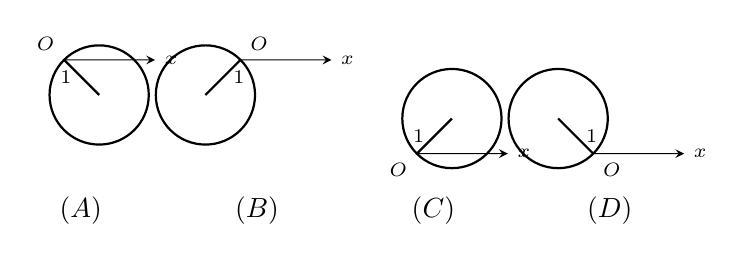
\begin{tikzpicture}[>=stealth, scale=0.70]
  \begin{scope}
    \coordinate (O) at (0,0.85);
    \coordinate (C) at (0.636,0.214);
    \draw[thick] (C) circle (0.9);
    \draw[thick] (O)--(C) node[midway, left, font=\scriptsize] {$1$};
    \draw[->] (O)--(1.65,0.85) node[right, font=\scriptsize] {$x$};
    \node[above left, font=\scriptsize] at (O) {$O$};
    \node[below] at (0.3,-1.45) {$(A)$};
  \end{scope}
  \begin{scope}[xshift=3.2cm]
    \coordinate (O) at (0,0.85);
    \coordinate (C) at (-0.636,0.214);
    \draw[thick] (C) circle (0.9);
    \draw[thick] (O)--(C) node[midway, right, font=\scriptsize] {$1$};
    \draw[->] (O)--(1.65,0.85) node[right, font=\scriptsize] {$x$};
    \node[above right, font=\scriptsize] at (O) {$O$};
    \node[below] at (0.3,-1.45) {$(B)$};
  \end{scope}
  \begin{scope}[xshift=6.4cm]
    \coordinate (O) at (0,-0.85);
    \coordinate (C) at (0.636,-0.214);
    \draw[thick] (C) circle (0.9);
    \draw[thick] (O)--(C) node[midway, left, font=\scriptsize] {$1$};
    \draw[->] (O)--(1.65,-0.85) node[right, font=\scriptsize] {$x$};
    \node[below left, font=\scriptsize] at (O) {$O$};
    \node[below] at (0.3,-1.45) {$(C)$};
  \end{scope}
  \begin{scope}[xshift=9.6cm]
    \coordinate (O) at (0,-0.85);
    \coordinate (C) at (-0.636,-0.214);
    \draw[thick] (C) circle (0.9);
    \draw[thick] (O)--(C) node[midway, right, font=\scriptsize] {$1$};
    \draw[->] (O)--(1.65,-0.85) node[right, font=\scriptsize] {$x$};
    \node[below right, font=\scriptsize] at (O) {$O$};
    \node[below] at (0.3,-1.45) {$(D)$};
  \end{scope}
\end{tikzpicture}
\end{center}
\nopagebreak[4]
\Needspace{4\baselineskip}
\textbf{解析}

\Needspace{5\baselineskip}
将极坐标方程化为直角坐标方程：

\nopagebreak[4]
\[
\rho=2\sin\left(\theta+\frac\pi4\right)
=\sqrt2(\sin\theta+\cos\theta).
\]

\Needspace{5\baselineskip}
两边乘以 $\rho$，得

\nopagebreak[4]
\[
x^2+y^2=\sqrt2(x+y),
\]

\Needspace{5\baselineskip}
即

\nopagebreak[4]
\[
\left(x-\frac{\sqrt2}{2}\right)^2
+\left(y-\frac{\sqrt2}{2}\right)^2=1.
\]

该圆心在第一象限，经过极点 $O$，且从 $O$ 沿正 $x$ 轴方向进入圆内，对照图形选 C。

\gkanswer{答案：C}

\end{answer}
\begin{answer}
\gksolhead{6}{}

\textbf{题目}：

函数 $y=\cos x+1\ (-\pi\le x\le0)$ 的反函数是\mbox{（　　）}

（A）$y=-\arccos(x-1)\ (0\le x\le2)$

（B）$y=\pi-\arccos(x-1)\ (0\le x\le2)$

（C）$y=\arccos(x-1)\ (0\le x\le2)$

（D）$y=\pi+\arccos(x-1)\ (0\le x\le2)$

\Needspace{4\baselineskip}
\textbf{解析}

\Needspace{5\baselineskip}
在 $[-\pi,0]$ 上，函数 $y=\cos x+1$ 的值域为 $[0,2]$，且反函数满足

\nopagebreak[4]
\[
x=\cos y+1,\qquad y\in[-\pi,0].
\]

\Needspace{5\baselineskip}
因此

\nopagebreak[4]
\[
y=-\arccos(x-1),\qquad 0\le x\le2.
\]

选 A。

\gkanswer{答案：A}

\end{answer}
\begin{answer}
\gksolhead{7}{}

\textbf{题目}：

若椭圆经过原点，且焦点为 $F_1(1,0)$、$F_2(3,0)$，则其离心率为\mbox{（　　）}

（A）$\dfrac34$　　（B）$\dfrac23$　　（C）$\dfrac12$　　（D）$\dfrac14$

\Needspace{4\baselineskip}
\textbf{解析}

\Needspace{5\baselineskip}
椭圆焦点的中点为中心 $(2,0)$，焦半距 $c=1$。因为椭圆经过原点，而原点到两个焦点的距离之和为 $1+3=4=2a$，所以 $a=2$。故离心率

\nopagebreak[4]
\[
e=\frac ca=\frac12.
\]

选 C。

\gkanswer{答案：C}

\end{answer}
\begin{answer}
\gksolhead{8}{}

\textbf{题目}：

若 $0<\alpha<\beta<\dfrac\pi4$，$\sin\alpha+\cos\alpha=a$，$\sin\beta+\cos\beta=b$，则\mbox{（　　）}

（A）$a>b$　　（B）$a<b$　　（C）$ab<1$　　（D）$ab>2$

\Needspace{4\baselineskip}
\textbf{解析}

\Needspace{5\baselineskip}
令 $h(t)=\sin t+\cos t$。在 $(0,\pi/4)$ 内，

\nopagebreak[4]
\[
h'(t)=\cos t-\sin t>0.
\]

由于 $0<\alpha<\beta<\pi/4$，有 $a=h(\alpha)<h(\beta)=b$，选 B。

\gkanswer{答案：B}

\end{answer}
\begin{answer}
\gksolhead{9}{}

\textbf{题目}：

在正三棱柱 $ABC-A_1B_1C_1$ 中，若 $AB=\sqrt2BB_1$，则 $AB_1$ 与 $C_1B$ 所成的角的大小为\mbox{（　　）}

（A）$60^\circ$　　（B）$90^\circ$　　（C）$45^\circ$　　（D）$120^\circ$

\Needspace{4\baselineskip}
\textbf{解析}

\Needspace{5\baselineskip}
设正三棱柱底面边长为 $s$，高为 $h$。由题设 $s=\sqrt2h$。取坐标

\nopagebreak[4]
\[
B=(0,0,0),\quad C=(s,0,0),\quad
A=\left(\frac s2,\frac{\sqrt3s}{2},0\right),
\]

\nopagebreak[4]
\[
B_1=(0,0,h),\quad C_1=(s,0,h).
\]

\Needspace{5\baselineskip}
则

\nopagebreak[4]
\[
\overrightarrow{AB_1}=\left(-\frac s2,-\frac{\sqrt3s}{2},h\right),
\qquad
\overrightarrow{BC_1}=(s,0,h).
\]

\Needspace{5\baselineskip}
其内积为

\nopagebreak[4]
\[
\overrightarrow{AB_1}\cdot\overrightarrow{BC_1}
=-\frac{s^2}{2}+h^2=0,
\]

故两直线垂直，所成角为 $90^\circ$，选 B。

\gkanswer{答案：B}

\end{answer}
\begin{answer}
\gksolhead{10}{}

\textbf{题目}：

设 $f(x)$、$g(x)$ 都是单调函数，有如下四个命题中，正确的命题是\mbox{（　　）}

① 若 $f(x)$ 单调递增，$g(x)$ 单调递增，则 $f(x)-g(x)$ 单调递增；

② 若 $f(x)$ 单调递增，$g(x)$ 单调递减，则 $f(x)-g(x)$ 单调递增；

③ 若 $f(x)$ 单调递减，$g(x)$ 单调递增，则 $f(x)-g(x)$ 单调递减；

④ 若 $f(x)$ 单调递减，$g(x)$ 单调递减，则 $f(x)-g(x)$ 单调递减。

（A）①③　　（B）①④　　（C）②③　　（D）②④

\Needspace{4\baselineskip}
\textbf{解析}

\Needspace{5\baselineskip}
若 $f$ 递增、$g$ 递减，则对 $x_1<x_2$ 有

\nopagebreak[4]
\[
f(x_1)<f(x_2),\qquad g(x_1)>g(x_2),
\]

从而 $f(x_1)-g(x_1)<f(x_2)-g(x_2)$，所以②正确。类似地，若 $f$ 递减、$g$ 递增，则 $f-g$ 递减，所以③正确；①、④均不能由已知推出。选 C。

\gkanswer{答案：C}

\end{answer}
\begin{answer}
\gksolhead{11}{}

\textbf{题目}：

一间民房的屋顶有如图三种不同的盖法：① 单向倾斜；② 双向倾斜；③ 四向倾斜。记三种盖法屋顶面积分别为 $P_1$、$P_2$、$P_3$。若屋顶斜面与水平面所成的角都是 $\alpha$，则\mbox{（　　）}
\nopagebreak[4]
\begin{center}% 2001 年全国旧课程卷理科第 11 题：三种屋顶盖法
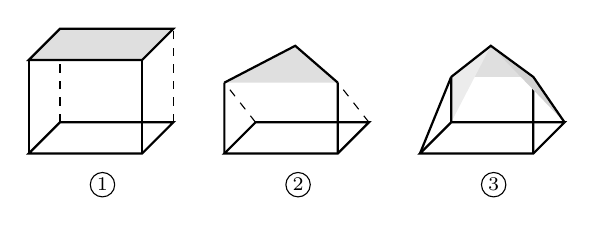
\begin{tikzpicture}[>=stealth, scale=0.72]
  \begin{scope}
    \coordinate (A) at (0,0);
    \coordinate (B) at (2.0,0);
    \coordinate (C) at (2.55,0.55);
    \coordinate (D) at (0.55,0.55);
    \coordinate (A1) at (0,1.65);
    \coordinate (B1) at (2.0,1.65);
    \coordinate (C1) at (2.55,2.2);
    \coordinate (D1) at (0.55,2.2);
    \draw[thick] (A)--(B)--(C)--(D)--cycle;
    \draw[thick] (A)--(A1) (B)--(B1);
    \draw[dashed] (C)--(C1) (D)--(D1);
    \fill[gray!25] (A1)--(B1)--(C1)--(D1)--cycle;
    \draw[thick] (A1)--(B1)--(C1)--(D1)--cycle;
    \node[circle,draw,inner sep=1pt] at (1.3,-0.55) {\scriptsize 1};
  \end{scope}
  \begin{scope}[xshift=3.45cm]
    \coordinate (A) at (0,0);
    \coordinate (B) at (2.0,0);
    \coordinate (C) at (2.55,0.55);
    \coordinate (D) at (0.55,0.55);
    \coordinate (M) at (1.25,1.9);
    \draw[thick] (A)--(B)--(C)--(D)--cycle;
    \draw[thick] (A)--(0,1.25) (B)--(2,1.25);
    \draw[dashed] (C)--(2,1.25) (D)--(0,1.25);
    \fill[gray!25] (0,1.25)--(M)--(2,1.25)--cycle;
    \draw[thick] (0,1.25)--(M)--(2,1.25);
    \node[circle,draw,inner sep=1pt] at (1.3,-0.55) {\scriptsize 2};
  \end{scope}
  \begin{scope}[xshift=6.9cm]
    \coordinate (A) at (0,0);
    \coordinate (B) at (2.0,0);
    \coordinate (C) at (2.55,0.55);
    \coordinate (D) at (0.55,0.55);
    \coordinate (M) at (1.25,1.9);
    \coordinate (L) at (0.55,1.35);
    \coordinate (R) at (2.0,1.35);
    \draw[thick] (A)--(B)--(C)--(D)--cycle;
    \draw[thick] (A)--(L) (B)--(R);
    \draw[dashed] (C)--(R) (D)--(L);
    \fill[gray!25] (L)--(M)--(R)--cycle;
    \fill[gray!15] (D)--(L)--(M)--cycle;
    \fill[gray!35] (M)--(R)--(C)--cycle;
    \draw[thick] (L)--(M)--(R) (D)--(L) (R)--(C);
    \node[circle,draw,inner sep=1pt] at (1.3,-0.55) {\scriptsize 3};
  \end{scope}
\end{tikzpicture}
\end{center}
\nopagebreak[4]
（A）$P_3>P_2>P_1$　　（B）$P_3>P_2=P_1$　　（C）$P_3=P_2>P_1$　　（D）$P_3=P_2=P_1$

\Needspace{4\baselineskip}
\textbf{解析}

\Needspace{5\baselineskip}
把每个屋顶斜面正投影到水平面。由于每个斜面与水平面的夹角都是 $\alpha$，斜面面积等于其水平投影面积除以 $\cos\alpha$。三种盖法覆盖的水平投影区域相同，因此三种屋顶总面积相等：

\nopagebreak[4]
\[
P_1=P_2=P_3.
\]

选 D。

\gkanswer{答案：D}

\end{answer}
\begin{answer}
\gksolhead{12}{}

\textbf{题目}：

如图，小圆圈表示网络的结点，结点之间的连线表示它们有网线相联。连线标注的数字表示该段网线单位时间内可以通过的最大信息量。现从结点 $A$ 向结点 $B$ 传递信息，信息可以分开沿不同的路线同时传递，则单位时间内传递的最大信息量为\mbox{（　　）}
\nopagebreak[4]
\begin{center}% 2001 年全国旧课程卷理科第 12 题：信息网络
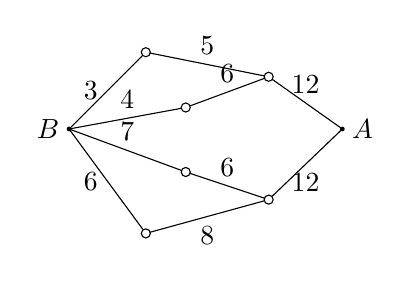
\begin{tikzpicture}[>=stealth, scale=0.78]
  \coordinate (B) at (0,0);
  \coordinate (U) at (1.25,1.25);
  \coordinate (V) at (3.25,0.85);
  \coordinate (M) at (1.9,0.35);
  \coordinate (N) at (1.9,-0.7);
  \coordinate (W) at (1.25,-1.7);
  \coordinate (Z) at (3.25,-1.15);
  \coordinate (A) at (4.45,0);

  \draw (B)--(U) node[midway, left] {3};
  \draw (U)--(V) node[midway, above] {5};
  \draw (B)--(M) node[midway, above] {4};
  \draw (M)--(V) node[midway, above] {6};
  \draw (B)--(N) node[midway, above] {7};
  \draw (N)--(Z) node[midway, above] {6};
  \draw (B)--(W) node[midway, left] {6};
  \draw (W)--(Z) node[midway, below] {8};
  \draw (V)--(A) node[midway, above] {12};
  \draw (Z)--(A) node[midway, below] {12};

  \foreach \point in {U,V,M,N,W,Z}
    \filldraw[fill=white] (\point) circle (2.1pt);
  \fill (B) circle (1.1pt) node[left] {$B$};
  \fill (A) circle (1.1pt) node[right] {$A$};
\end{tikzpicture}
\end{center}
\nopagebreak[4]
（A）$26$　　（B）$24$　　（C）$20$　　（D）$19$

\Needspace{4\baselineskip}
\textbf{解析}

虽然题面叙述传输方向为 $A$ 到 $B$，把所有边方向反向后容量问题等价；下面按图中从 $B$ 到 $A$ 计。将网络分成上、下两部分。上部从 $B$ 出发的两条边容量为 $3,4$，故上部最多传递 $7$；这 $7$ 单位可以分别沿容量为 $5,6$ 的边汇合后经容量为 $12$ 的边传到 $A$。

\Needspace{5\baselineskip}
下部汇合到右下结点的出口容量为 $12$，且可由 $B$ 到下部的容量 $7,6$ 及中间容量 $6,8$ 的边提供足够流量，所以可传递 $12$。因此总流量不超过

\nopagebreak[4]
\[
7+12=19.
\]

取上部流量 $3+4=7$，下部令两条支路各传 $6$，恰好得到总流量 $19$，故最大信息量为 $19$，选 D。

\gkanswer{答案：D}

\end{answer}
\gkpart{二、填空题}

\begin{answer}
\gksolhead{13}{}

\textbf{题目}：

若一个圆锥的轴截面是等边三角形，其面积为 $\sqrt3$，则这个圆锥的侧面积是\gkblank{}。

\Needspace{4\baselineskip}
\textbf{解析}

\Needspace{5\baselineskip}
设圆锥轴截面为边长 $\ell$ 的等边三角形。由面积条件

\nopagebreak[4]
\[
\frac{\sqrt3}{4}\ell^2=\sqrt3,\qquad \ell=2.
\]

\Needspace{5\baselineskip}
轴截面的底边是圆锥底面直径，所以底面半径 $r=1$；轴截面的两腰是母线，母线长 $l=2$。故圆锥侧面积为

\nopagebreak[4]
\[
S_{\text{\text{侧}}}=\pi r l=2\pi.
\]

\gkanswer{答案：$2\pi$}

\end{answer}
\begin{answer}
\gksolhead{14}{}

\textbf{题目}：

双曲线 $\dfrac{x^2}{9}-\dfrac{y^2}{16}=1$ 的两个焦点为 $F_1,F_2$，点 $P$ 在双曲线上，若 $PF_1\perp PF_2$，则点 $P$ 到 $x$ 轴的距离为\gkblank{}。

\Needspace{4\baselineskip}
\textbf{解析}

\Needspace{5\baselineskip}
双曲线焦点为 $F_1(-5,0),F_2(5,0)$。设 $P=(x,y)$，由 $PF_1\perp PF_2$ 得

\nopagebreak[4]
\[
(x+5,y)\cdot(x-5,y)=0,\qquad x^2+y^2=25.
\]

\Needspace{5\baselineskip}
又因为 $P$ 在双曲线上，

\nopagebreak[4]
\[
\frac{x^2}{9}-\frac{y^2}{16}=1.
\]

\Needspace{5\baselineskip}
联立 $x^2+y^2=25$，得到

\nopagebreak[4]
\[
16x^2-9y^2=144,\qquad
16(25-y^2)-9y^2=144,
\]

\Needspace{5\baselineskip}
即 $25y^2=256$。所以点 $P$ 到 $x$ 轴的距离为

\nopagebreak[4]
\[
|y|=\frac{16}{5}.
\]

\gkanswer{答案：$\dfrac{16}{5}$}

\end{answer}
\begin{answer}
\gksolhead{15}{}

\textbf{题目}：

设 $\{a_n\}$ 是公比为 $q$ 的等比数列，$S_n$ 是它的前 $n$ 项和。若 $\{S_n\}$ 是等差数列，则 $q=$\gkblank{}。

\Needspace{4\baselineskip}
\textbf{解析}

\Needspace{5\baselineskip}
因为 $S_{n+1}-S_n=a_{n+1}$，若 $\{S_n\}$ 为等差数列，则 $a_{n+1}$ 为常数。按等比数列的定义，公比 $q\ne0$ 且各项可作相邻项之比，所以 $a_2\ne0$；由 $a_2=a_3$ 得

\nopagebreak[4]
\[
a_2q=a_2,\qquad q=1.
\]

\gkanswer{答案：$q=1$}

\end{answer}
\begin{answer}
\gksolhead{16}{}

\textbf{题目}：

圆周上有 $2n$ 个等分点（$n>1$），以其中三个点为顶点的直角三角形的个数为\gkblank{}。

\Needspace{4\baselineskip}
\textbf{解析}

\Needspace{5\baselineskip}
圆内接三角形为直角三角形，当且仅当其斜边为圆的直径。$2n$ 个等分点两两关于圆心对称，共有 $n$ 条直径。固定一条直径的两个端点后，第三个顶点可从其余 $2n-2$ 个点中任选一个，且每个直角三角形的斜边唯一确定。因此个数为

\nopagebreak[4]
\[
n(2n-2)=2n(n-1).
\]

\gkanswer{答案：$2n(n-1)$}

\end{answer}
\gkpart{三、解答题}

\begin{answer}
\gksolhead{17}{}

\textbf{题目}：

如图，在底面是直角梯形的四棱锥 $S-ABCD$ 中，$\angle ABC=90^\circ$，$SA\perp$ 面 $ABCD$，$SA=AB=BC=1$，$AD=\dfrac12$。
\nopagebreak[4]
\begin{center}% 2001 年全国旧课程卷理科第 17 题：直角梯形底面的四棱锥
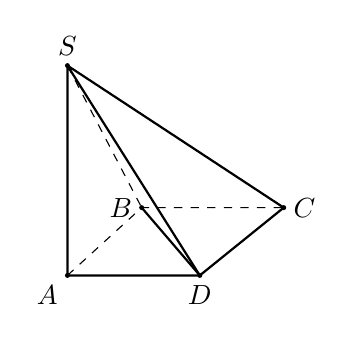
\begin{tikzpicture}[>=stealth, scale=0.82]
  \coordinate (A) at (0,0);
  \coordinate (B) at (1.15,1.05);
  \coordinate (C) at (3.35,1.05);
  \coordinate (D) at (2.05,0);
  \coordinate (S) at (0,3.25);

  \draw[thick] (S)--(A) (S)--(C) (S)--(D);
  \draw[dashed] (S)--(B);
  \draw[thick] (A)--(D)--(C);
  \draw[dashed] (A)--(B)--(C);
  \draw[thick] (B)--(D);

  \fill (S) circle (1.1pt) node[above] {$S$};
  \fill (A) circle (1.1pt) node[below left] {$A$};
  \fill (B) circle (1.1pt) node[left] {$B$};
  \fill (C) circle (1.1pt) node[right] {$C$};
  \fill (D) circle (1.1pt) node[below] {$D$};
\end{tikzpicture}
\end{center}
\nopagebreak[4]
（1） 求四棱锥 $S-ABCD$ 的体积；

（2） 求面 $SCD$ 与面 $SBA$ 所成的二面角的正切值。

\Needspace{4\baselineskip}
\textbf{解析}

\Needspace{5\baselineskip}
取底面为 $z=0$，令

\nopagebreak[4]
\[
B=(0,0,0),\quad C=(1,0,0),\quad A=(0,1,0),\quad
D=\left(\frac12,1,0\right),\quad S=(0,1,1).
\]

这满足 $AD\parallel BC$、$\angle ABC=90^\circ$ 以及题设各长度。

\gksubpart{(1)}

\Needspace{5\baselineskip}
底面直角梯形 $ABCD$ 的面积为

\nopagebreak[4]
\[
S_{ABCD}=\frac{(AD+BC)\cdot AB}{2}
=\frac{\left(\frac12+1\right)\cdot1}{2}=\frac34.
\]

\Needspace{5\baselineskip}
四棱锥的高为 $SA=1$，故体积

\nopagebreak[4]
\[
V=\frac13S_{ABCD}\cdot SA=\frac14.
\]

\gksubpart{(2)}

\Needspace{5\baselineskip}
平面 $SBA$ 的方程为 $x=0$，可取法向量

\nopagebreak[4]
\[
\boldsymbol n_1=(1,0,0).
\]

\Needspace{5\baselineskip}
平面 $SCD$ 中

\nopagebreak[4]
\[
\overrightarrow{SC}=(1,-1,-1),\qquad
\overrightarrow{SD}=\left(\frac12,0,-1\right),
\]

\Needspace{5\baselineskip}
故可取法向量

\nopagebreak[4]
\[
\boldsymbol n_2=\overrightarrow{SC}\times\overrightarrow{SD}
=\left(1,\frac12,\frac12\right).
\]

\Needspace{5\baselineskip}
设两平面所成的锐二面角为 $\varphi$，则

\nopagebreak[4]
\[
\cos\varphi=\frac{|\boldsymbol n_1\cdot\boldsymbol n_2|}
{|\boldsymbol n_1|\,|\boldsymbol n_2|}
=\frac1{\sqrt6/2}=\sqrt{\frac23}.
\]

\Needspace{5\baselineskip}
于是

\nopagebreak[4]
\[
\tan\varphi=\sqrt{\frac1{\cos^2\varphi}-1}
=\sqrt{\frac32-1}=\frac{\sqrt2}{2}.
\]

\gkanswer{答案（1）：$\dfrac14$。}

\gkanswer{答案（2）：$\dfrac{\sqrt2}{2}$。}

\end{answer}
\begin{answer}
\gksolhead{18}{}

\textbf{题目}：

已知复数 $z_1=i(1-i)^3$。

（1） 求 $\arg z_1$ 及 $|z_1|$；

（2） 当复数 $z$ 满足 $|z|=1$，求 $|z-z_1|$ 的最大值。

\Needspace{4\baselineskip}
\textbf{解析}

\Needspace{5\baselineskip}
先计算

\nopagebreak[4]
\[
(1-i)^2=-2i,\qquad (1-i)^3=-2-2i,
\]

\Needspace{5\baselineskip}
从而

\nopagebreak[4]
\[
z_1=i(1-i)^3=2-2i.
\]

\gksubpart{(1)}

\Needspace{5\baselineskip}
因此 $z_1$ 位于第四象限，

\nopagebreak[4]
\[
\arg z_1=-\frac\pi4,\qquad |z_1|=\sqrt{2^2+(-2)^2}=2\sqrt2.
\]

\gksubpart{(2)}

\Needspace{5\baselineskip}
在复平面内，$|z|=1$ 表示以原点为圆心、半径为 $1$ 的圆。由三角不等式

\nopagebreak[4]
\[
|z-z_1|\le |z|+|z_1|=1+2\sqrt2.
\]

\Needspace{5\baselineskip}
当 $z$ 与 $z_1$ 方向相反时取等号，故最大值为

\nopagebreak[4]
\[
1+2\sqrt2.
\]

\gkanswer{答案（1）：$\arg z_1=-\dfrac\pi4$，$|z_1|=2\sqrt2$。}

\gkanswer{答案（2）：$1+2\sqrt2$。}

\end{answer}
\begin{answer}
\gksolhead{19}{}

\textbf{题目}：

设抛物线 $y^2=2px\ (p>0)$ 的焦点为 $F$，经过点 $F$ 的直线交抛物线于 $A$、$B$ 两点。点 $C$ 在抛物线的准线上，且 $BC\parallel x$ 轴。证明直线 $AC$ 经过原点 $O$。

\Needspace{4\baselineskip}
\textbf{解析}

\Needspace{5\baselineskip}
令 $a=\dfrac p2$，则抛物线可参数表示为

\nopagebreak[4]
\[
P(t)=(at^2,2at),
\]

\Needspace{5\baselineskip}
其焦点为 $F=(a,0)$。设 $A=P(t_1)$、$B=P(t_2)$。过参数为 $t_1,t_2$ 两点的弦方程为

\nopagebreak[4]
\[
2x-(t_1+t_2)y+2at_1t_2=0.
\]

\Needspace{5\baselineskip}
因为该弦经过焦点 $F$，代入得

\nopagebreak[4]
\[
2a+2at_1t_2=0,\qquad t_1t_2=-1.
\]

\Needspace{5\baselineskip}
抛物线准线为 $x=-a$。点 $C$ 在准线上，且 $BC\parallel x$ 轴，所以

\nopagebreak[4]
\[
C=(-a,2at_2).
\]

\Needspace{5\baselineskip}
又 $t_1=-1/t_2$，故

\nopagebreak[4]
\[
A=\left(\frac a{t_2^2},-\frac{2a}{t_2}\right).
\]

\Needspace{5\baselineskip}
于是

\nopagebreak[4]
\[
\det\begin{pmatrix}
x_A & y_A\\
x_C & y_C
\end{pmatrix}
=\frac a{t_2^2}\cdot2at_2
-\left(-\frac{2a}{t_2}\right)(-a)=0.
\]

所以 $O,A,C$ 三点共线，直线 $AC$ 经过原点 $O$。

\gkanswer{答案：证明见解析版。}

\end{answer}
\begin{answer}
\gksolhead{20}{}

\textbf{题目}：

已知 $i,m,n$ 是正整数，且 $1<i\le m<n$。

（1） 证明：$n^iA_m^i<m^iA_n^i$；

（2） 证明：$(1+m)^n>(1+n)^m$。

\Needspace{4\baselineskip}
\textbf{解析}

\Needspace{5\baselineskip}
记

\nopagebreak[4]
\[
A_m^i=m(m-1)\cdots(m-i+1).
\]

\gksubpart{(1)}

\Needspace{5\baselineskip}
由于 $n>m$，对 $k=1,2,\ldots,i-1$ 有

\nopagebreak[4]
\[
\frac{n-k}{m-k}>\frac nm,
\]

\Needspace{5\baselineskip}
且第一项对应 $k=0$ 时等号成立。因此 $i>1$ 时

\nopagebreak[4]
\[
\frac{A_n^i}{A_m^i}
=\prod_{k=0}^{i-1}\frac{n-k}{m-k}
>\left(\frac nm\right)^i.
\]

\Needspace{5\baselineskip}
整理得

\nopagebreak[4]
\[
n^iA_m^i<m^iA_n^i.
\]

\gksubpart{(2)}

\Needspace{5\baselineskip}
令

\nopagebreak[4]
\[
h(x)=\frac{\ln(1+x)}x,\qquad x>0.
\]

\Needspace{5\baselineskip}
则

\nopagebreak[4]
\[
h'(x)=\frac{\frac{x}{1+x}-\ln(1+x)}{x^2}<0,
\]

\Needspace{5\baselineskip}
因为

\nopagebreak[4]
\[
\ln(1+x)=\int_0^x\frac{dt}{1+t}>\frac{x}{1+x}.
\]

\Needspace{5\baselineskip}
所以 $h(x)$ 在正数上递减。由 $m<n$，得

\nopagebreak[4]
\[
\frac{\ln(1+m)}m>\frac{\ln(1+n)}n.
\]

\Needspace{5\baselineskip}
两边乘以 $mn$，得到

\nopagebreak[4]
\[
n\ln(1+m)>m\ln(1+n),
\]

\Needspace{5\baselineskip}
从而

\nopagebreak[4]
\[
(1+m)^n>(1+n)^m.
\]

\gkanswer{答案（1）：证明见解析版。}

\gkanswer{答案（2）：证明见解析版。}

\end{answer}
\begin{answer}
\gksolhead{21}{}

\textbf{题目}：

从社会效益和经济效益出发，某地投入资金进行生态环境建设，并以此发展旅游产业。根据规划，本年度投入 $800$ 万元，以后每年投入将比上年减少 $\dfrac15$。本年度当地旅游业收入估计为 $400$ 万元，由于该项建设对旅游业的促进作用，预计今后的旅游业收入每年会比上年增加 $\dfrac14$。

（1） 设 $n$ 年内（本年度为第一年）总投入为 $a_n$ 万元，旅游业总收入为 $b_n$ 万元。写出 $a_n$、$b_n$ 的表达式；

（2） 至少经过几年旅游业的总收入才能超过总投入？

\Needspace{4\baselineskip}
\textbf{解析}

\gksubpart{(1)}

\Needspace{5\baselineskip}
每年投入构成首项为 $800$、公比为 $4/5$ 的等比数列，因此

\nopagebreak[4]
\[
a_n=800\frac{1-(4/5)^n}{1-4/5}
=4000\left[1-\left(\frac45\right)^n\right].
\]

\Needspace{5\baselineskip}
每年旅游业收入构成首项为 $400$、公比为 $5/4$ 的等比数列，因此

\nopagebreak[4]
\[
b_n=400\frac{(5/4)^n-1}{5/4-1}
=1600\left[\left(\frac54\right)^n-1\right].
\]

\gksubpart{(2)}

\Needspace{5\baselineskip}
令 $x=(5/4)^n$，则 $(4/5)^n=1/x$。由 $b_n>a_n$ 得

\nopagebreak[4]
\[
1600(x-1)>4000\left(1-\frac1x\right).
\]

\Needspace{5\baselineskip}
因 $x>1$，化简为

\nopagebreak[4]
\[
4x(x-1)>10(x-1),\qquad x>\frac52.
\]

当 $n=4$ 时 $(5/4)^4=625/256<5/2$；当 $n=5$ 时 $(5/4)^5=3125/1024>5/2$。故至少经过 $5$ 年。

\gkanswer{答案（1）：$a_n=4000\left[1-\left(\dfrac45\right)^n\right]$，$b_n=1600\left[\left(\dfrac54\right)^n-1\right]$。}

\gkanswer{答案（2）：至少经过 $5$ 年。}

\end{answer}
\begin{answer}
\gksolhead{22}{}

\textbf{题目}：

设 $f(x)$ 是定义在 $\mathbb R$ 上的偶函数，其图象关于直线 $x=1$ 对称。对任意 $x_1,x_2\in\left[0,\dfrac12\right]$，都有 $f(x_1+x_2)=f(x_1)\cdot f(x_2)$，且 $f(1)=a>0$。

（1） 求 $f\left(\dfrac12\right),f\left(\dfrac14\right)$；

（2） 证明：$f(x)$ 是周期函数；

（3） 记 $a_n=f\left(2n+\dfrac1{2n}\right)$，求 $\displaystyle\lim_{n\to\infty}\ln a_n$。

\Needspace{4\baselineskip}
\textbf{解析}

\gksubpart{(1)}

\Needspace{5\baselineskip}
令题设乘法关系中的 $x_1=x_2=1/2$，得

\nopagebreak[4]
\[
f(1)=f\left(\frac12\right)^2=a.
\]

\Needspace{5\baselineskip}
又令 $x_1=x_2=1/4$，有

\nopagebreak[4]
\[
f\left(\frac12\right)=f\left(\frac14\right)^2.
\]

\Needspace{5\baselineskip}
由于对区间内的任意 $x$ 都有 $f(x)=f(x/2)^2\ge0$，且 $f(1/2)^2=a>0$，所以取正平方根：

\nopagebreak[4]
\[
f\left(\frac12\right)=\sqrt a,\qquad
f\left(\frac14\right)=\sqrt[4]{a}.
\]

\gksubpart{(2)}

\Needspace{5\baselineskip}
图象关于直线 $x=1$ 对称，故对任意 $x$ 有

\nopagebreak[4]
\[
f(2-x)=f(x).
\]

\Needspace{5\baselineskip}
函数为偶函数，所以

\nopagebreak[4]
\[
f(x+2)=f\bigl(2-(-x)\bigr)=f(-x)=f(x).
\]

因此 $2$ 是 $f(x)$ 的一个周期，$f(x)$ 是周期函数。

\gksubpart{(3)}

\Needspace{5\baselineskip}
由周期性，

\nopagebreak[4]
\[
a_n=f\left(2n+\frac1{2n}\right)=f\left(\frac1{2n}\right).
\]

\Needspace{5\baselineskip}
把 $1/(2n)$ 连加 $n$ 次，利用题设乘法关系逐次得到

\nopagebreak[4]
\[
f\left(\frac12\right)=f\left(\frac1{2n}\right)^n.
\]

\Needspace{5\baselineskip}
由于 $f(1/(2n))\ge0$，且左端为正，故

\nopagebreak[4]
\[
a_n=f\left(\frac1{2n}\right)=a^{1/(2n)}.
\]

\Needspace{5\baselineskip}
于是

\nopagebreak[4]
\[
\lim_{n\to\infty}\ln a_n
=\lim_{n\to\infty}\frac{\ln a}{2n}=0.
\]

\gkanswer{答案（1）：$f\left(\dfrac12\right)=\sqrt a$，$f\left(\dfrac14\right)=\sqrt[4]{a}$。}

\gkanswer{答案（2）：$2$ 是 $f(x)$ 的一个周期。}

\gkanswer{答案（3）：$0$。}

\end{answer}